\chapter{Methodology}
\label{ch:method}

This chapter details the methodology employed to analyze and optimize the transportation network for students of the Izmir Institute of Technology residing in Izmir. The primary objective is to identify efficient bus routing strategies that minimize overall fuel consumption while adhering to practical constraints on bus capacity. Specifically, the network serves approximately 2000 students, and routes must accommodate a minimum of 10 and a maximum of 50 students per vehicle. 

Our approach leverages graph theory, treating student locations as nodes and potential travel segments as edges. We systematically explore various graph construction techniques and clustering algorithms to model the spatial relationships and identify optimal bus routes. The methodology is divided into three main sections: graph representation of the transportation map, clustering of the graph representations, and robustness analysis for the clustering solutions.

\section{Graph Representation of Transportation Map of IZTECH}
\label{sec:graph_representation}

The foundation of our analysis is a dataset comprising the geographical coordinates of approximately 2000 students located throughout the Izmir metropolitan area. In our graph-based model, each student's location is represented as a distinct node (or vertex) $v$ within a set $V$. The set $V$ thus encapsulates all student locations considered in the transportation network, where $|V| \approx 2000$. 

% Placeholder for Map Visualization
\begin{figure}[!htbp]
\centering
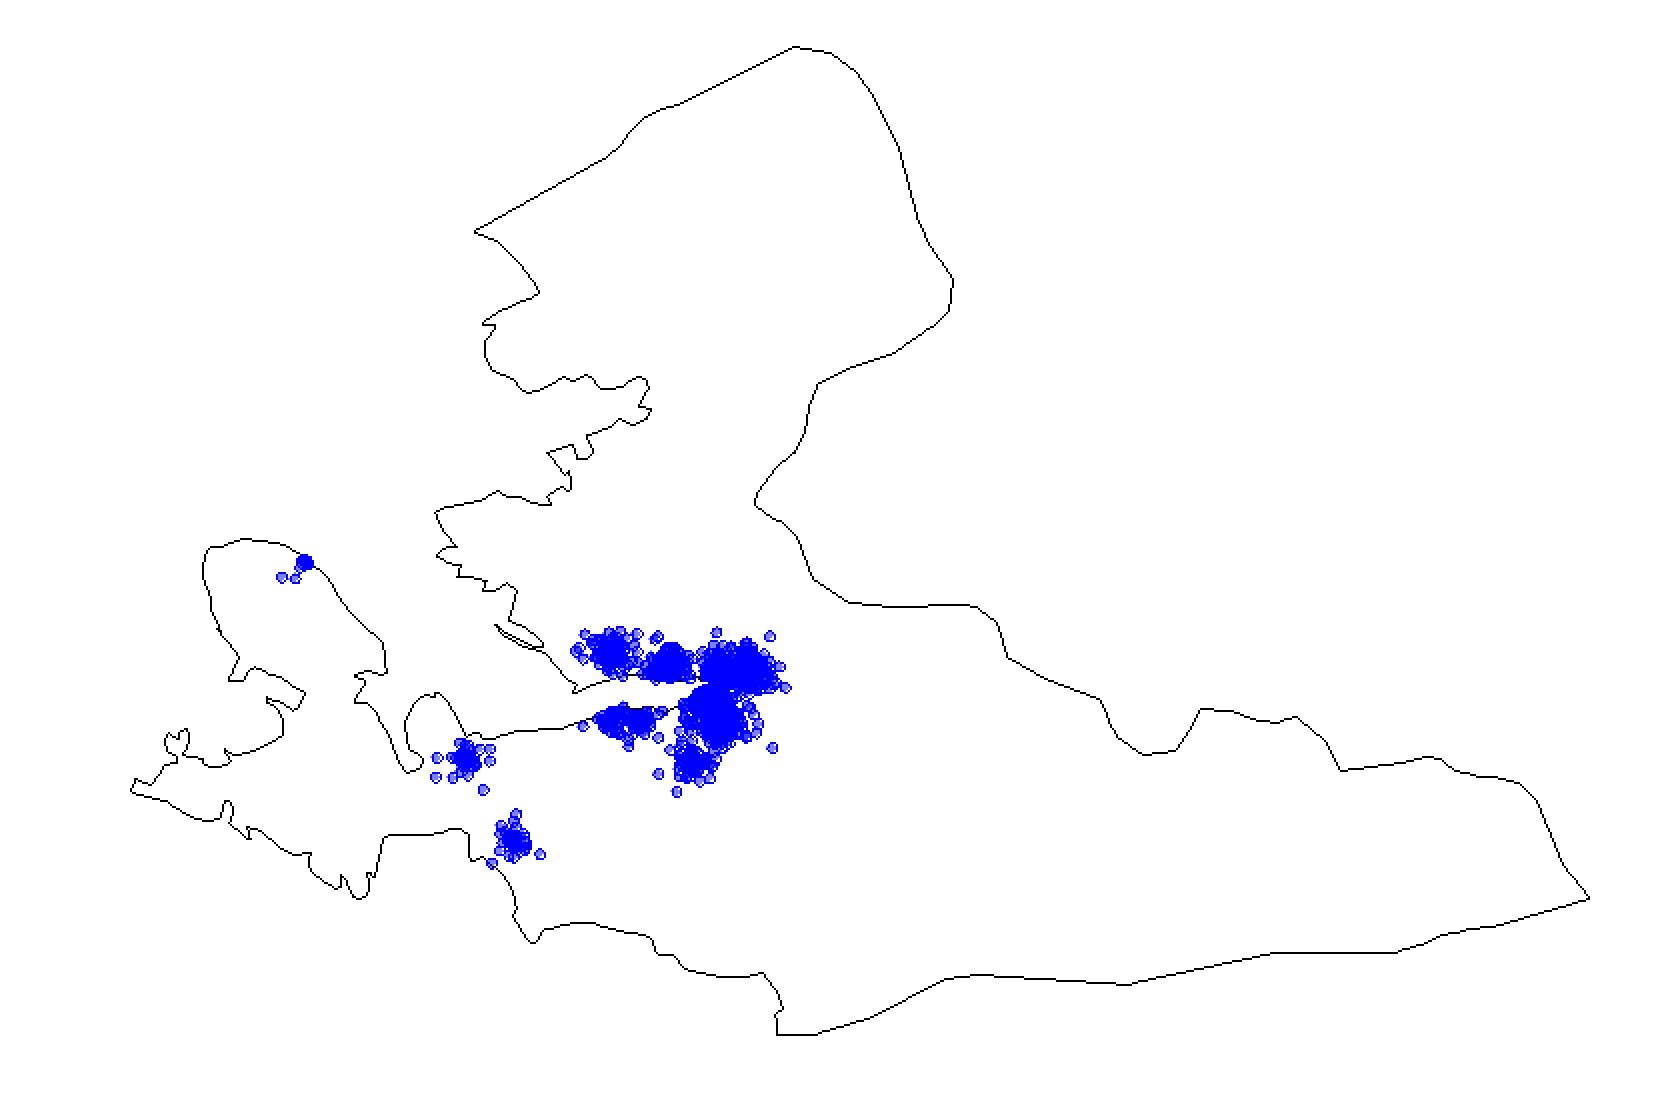
\includegraphics[width=0.8\textwidth]{img/student_map}
\caption{Geographical distribution of student locations in Izmir.}
\label{fig:student_map}
\end{figure}

\subsection{Complete Graph Representation}
\label{subsec:complete_graph}

The complete graph connects every pair of distinct student locations, representing maximum potential connectivity as detailed in Section~\ref{subsec:GraphConstructionMethods}. Edge weights $w_{uv}$ represent the estimated travel cost between locations $u$ and $v$.

This representation serves as our baseline model, establishing upper bounds on connectivity. However, the dense connectivity often leads to suboptimal routing solutions with higher overall costs due to the ${|V| \choose 2}$ edges making it computationally expensive for large datasets.

\subsubsection{Minibus Solution for Imbalanced Clusters}
\label{subsubsec:minibus_solution}

When analyzing the complete graph representation, we observed that the resulting clusters were often imbalanced, with many clusters having fewer than 25 students. This created an inefficiency in the transportation system, as standard buses with a capacity of 50 students would be underutilized.

To address this issue, we implemented a vehicle type allocation strategy that assigns minibuses (with a maximum capacity of 25 students) to smaller clusters and standard buses to larger ones:

\begin{itemize}
    \item Clusters with 10-25 students: Assigned to minibuses
    \item Clusters with 26-50 students: Assigned to standard buses
\end{itemize}

This differentiated approach resulted in significant cost savings due to the lower fuel consumption of minibuses compared to standard buses. However, it's important to note that IZTECH currently does not have minibuses in its fleet, only standard buses. This limitation motivates our exploration of alternative graph construction methods that might produce more balanced clusters suitable for the existing bus fleet.

\subsection{Sparse Graph Representation}
\label{subsec:sparse_graph}

Given the computational and practical limitations of the complete graph approach, we explored several sparse graph construction techniques that preserve essential connectivity while significantly reducing the number of edges. These methods emphasize local connections and spatial proximity, resulting in more efficient representations of the transportation network.

\subsubsection{Delaunay Graph Representation}
\label{subsubsec:delaunay}

The Delaunay triangulation constructs a graph based on the empty circumcircle property as explained in Section~\ref{subsec:GraphConstructionMethods}, creating a planar graph that avoids edge crossings.

In our implementation, we utilized the JTS Topology Suite to create the Delaunay triangulation of student locations. This representation naturally connects nearby points while avoiding edge crossings, which can represent physical barriers or inefficient routes. Our implementation assigns edge weights based on the Euclidean distance between connected nodes, approximating the fuel cost for direct travel.

\subsubsection{Gabriel Graph Representation}
\label{subsubsec:gabriel}

The Gabriel graph is a subgraph of the Delaunay triangulation that connects nodes if the circle with diameter between them contains no other nodes, as described in Section~\ref{subsec:GraphConstructionMethods}.

Our implementation constructs the Gabriel graph by first generating the Delaunay triangulation and then filtering edges based on the empty circle criterion. This approach preserves the most efficient local connections while further reducing the computational complexity compared to the complete graph.

\subsubsection{K-Nearest Neighbour Graph Representation}
\label{subsubsec:knn}

The K-Nearest Neighbors (KNN) graph connects each node to its $k$ closest neighbors, creating a sparse representation that emphasizes local connectivity as detailed in Section~\ref{subsec:GraphConstructionMethods}.

In our implementation, we dynamically determine an appropriate value of $k$ based on the network size and density, ensuring sufficient connectivity while maintaining computational efficiency. The graph is constructed using spatial indexing for efficient neighbor queries, with edge weights based on the Euclidean distance between connected nodes.

% Placeholder for Graph Examples Visualization
\begin{figure}[!htbp]
\centerline{
\subfigure[Complete Graph]{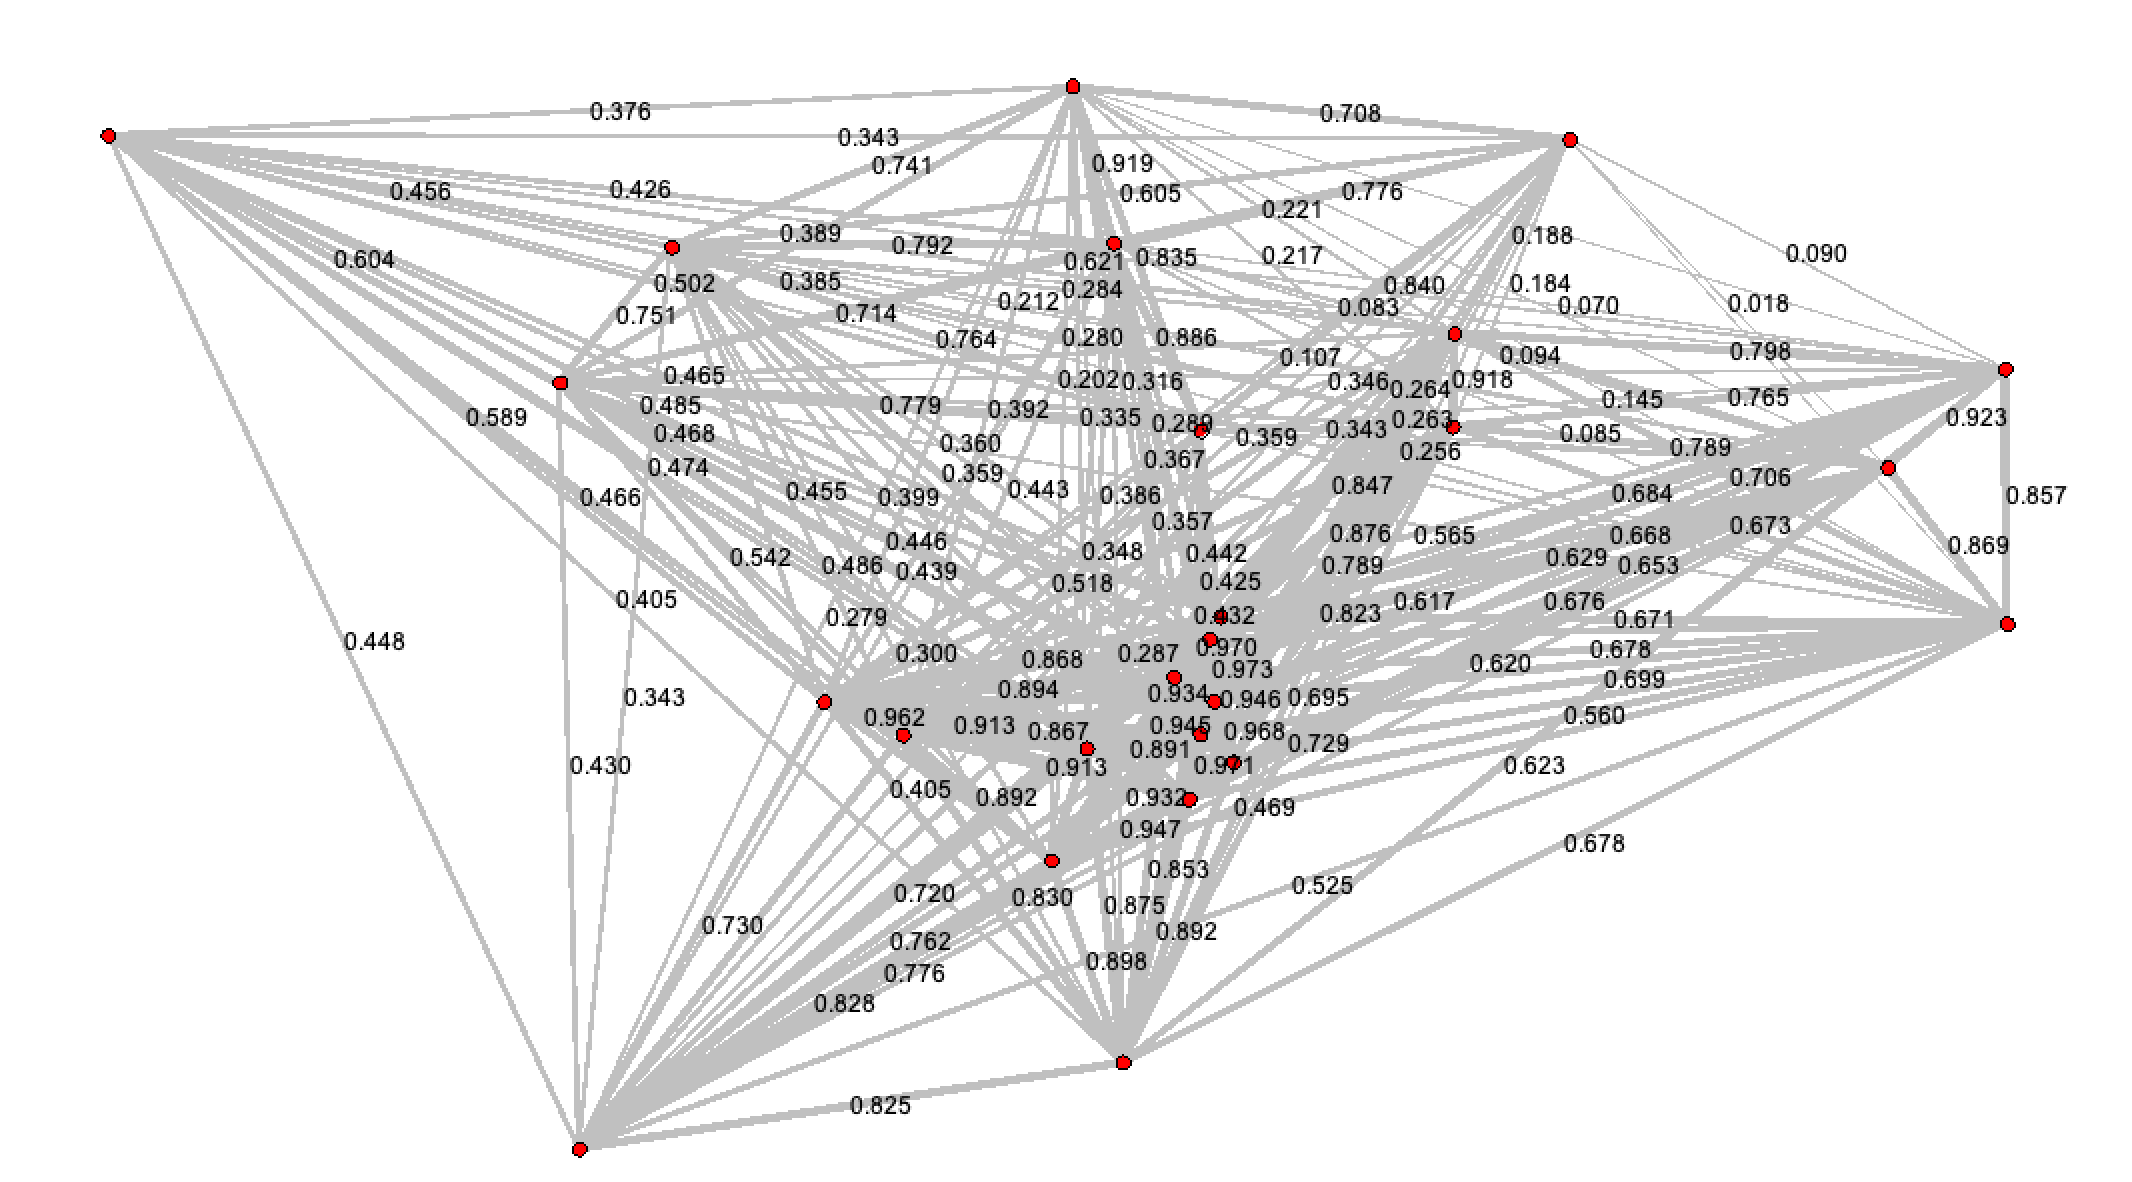
\includegraphics[width=0.45\textwidth]{img/complete}}
\subfigure[K-Nearest Neighbors ($k=5$)]{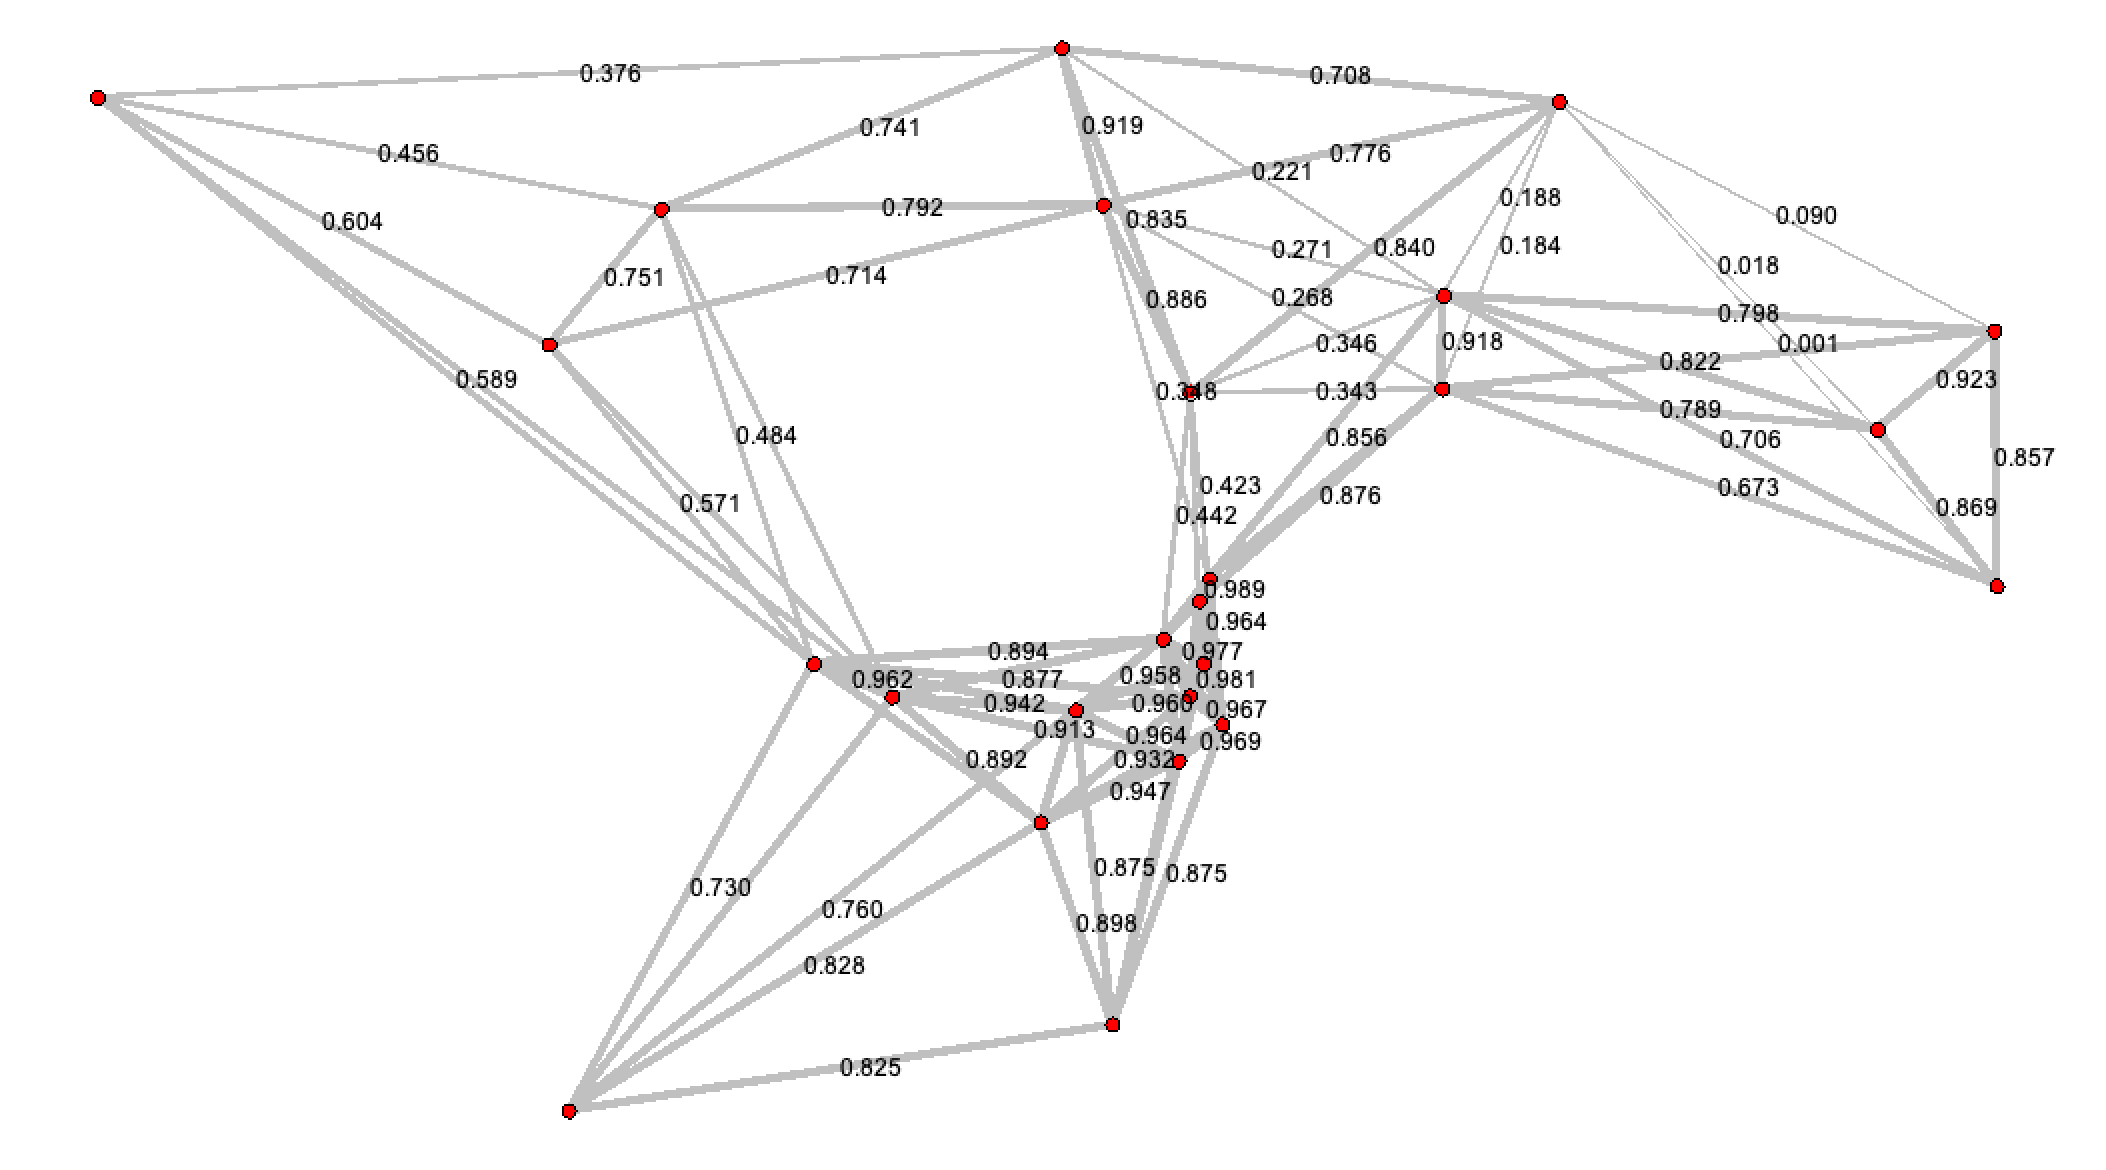
\includegraphics[width=0.45\textwidth]{img/k_nearest}}
}
\centerline{
\subfigure[Delaunay Triangulation]{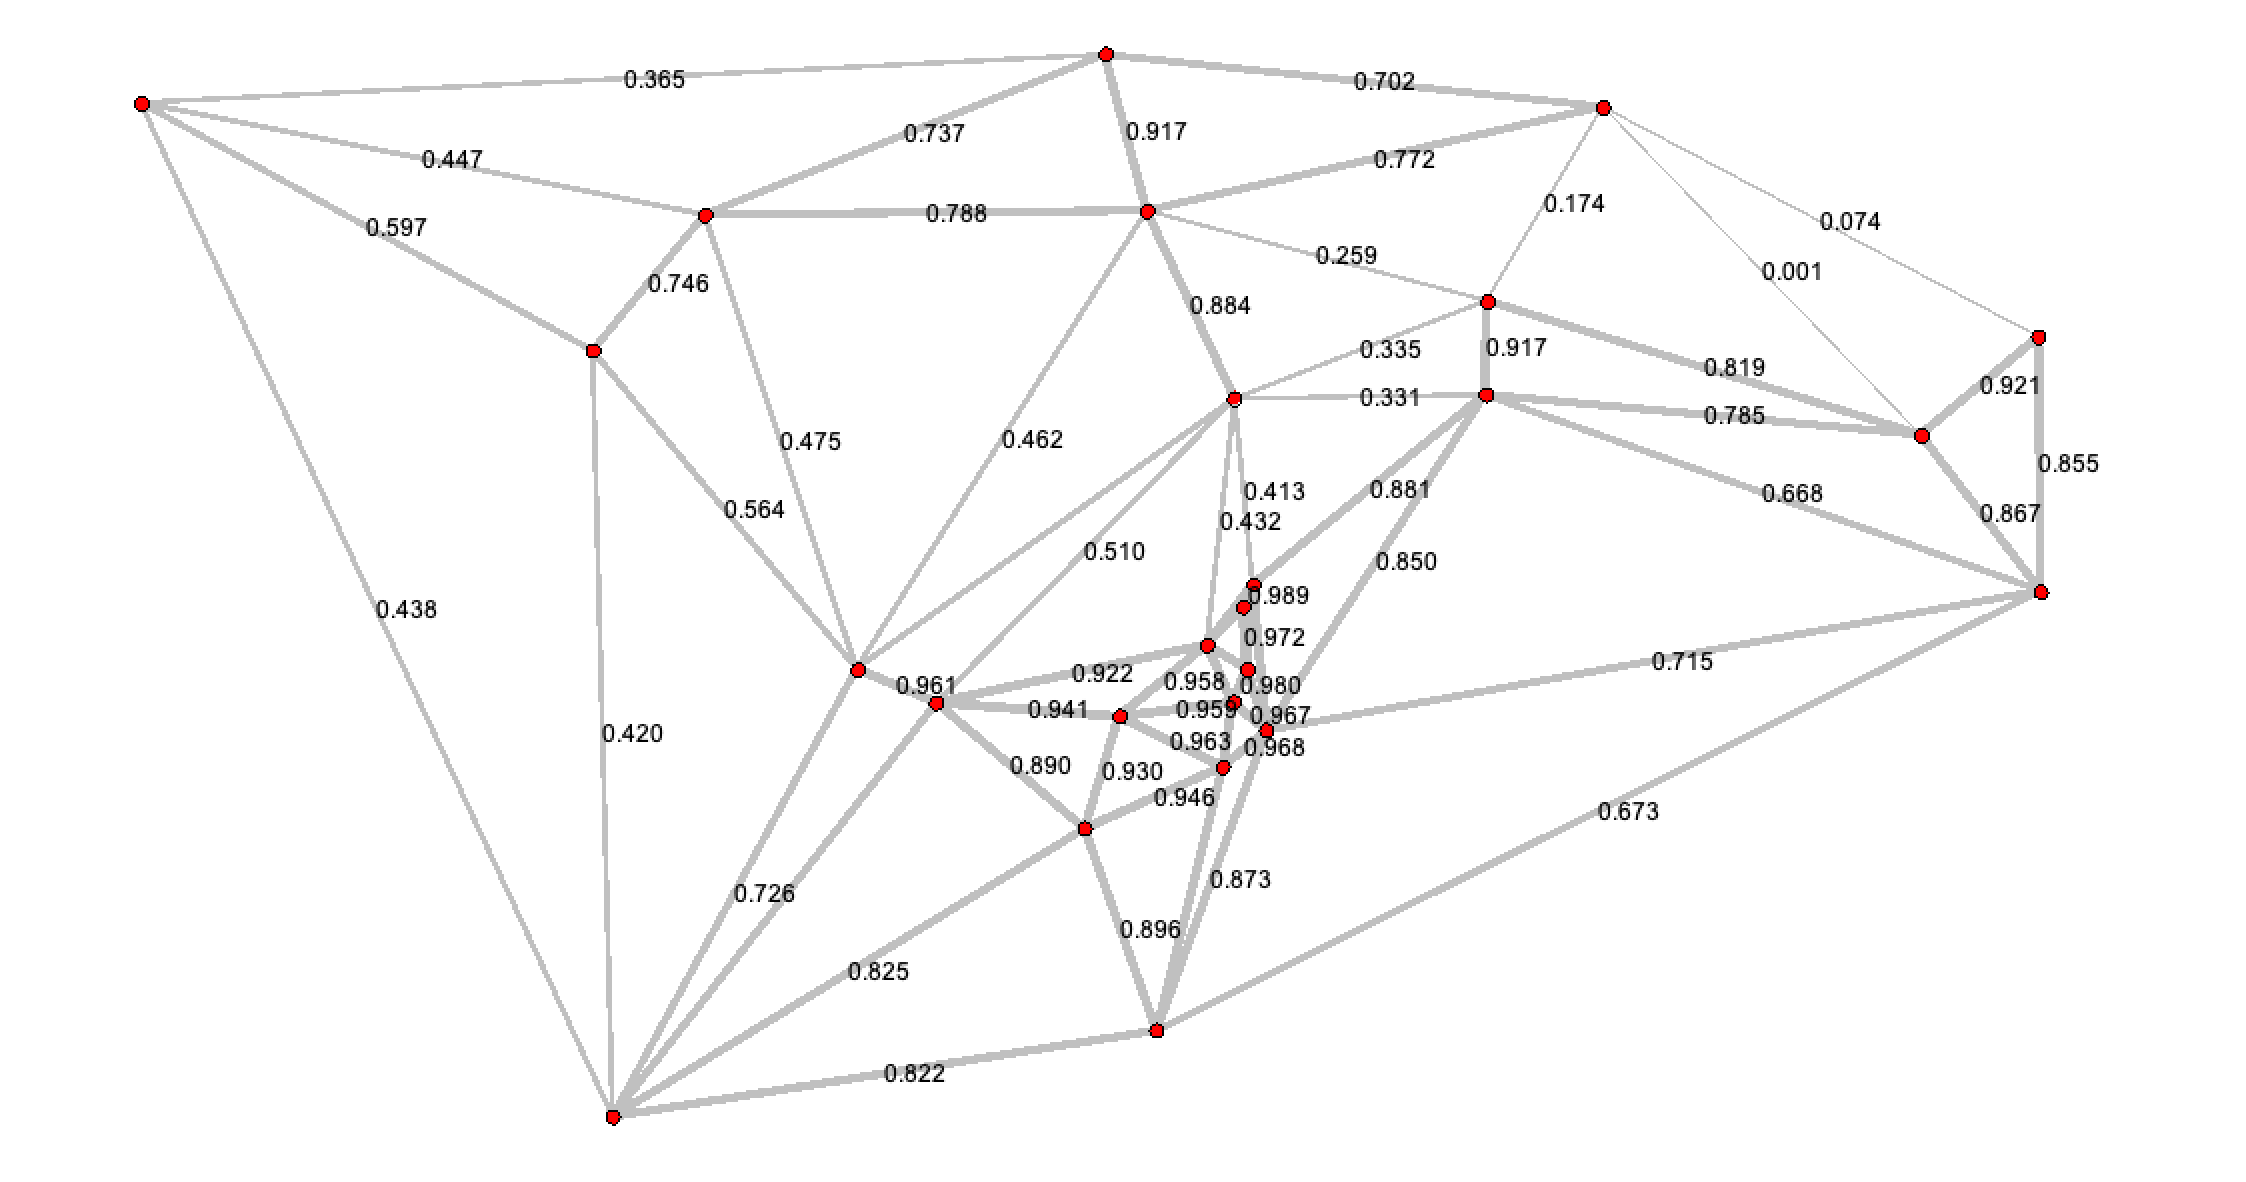
\includegraphics[width=0.45\textwidth]{img/delaunay}}
\subfigure[Gabriel Graph]{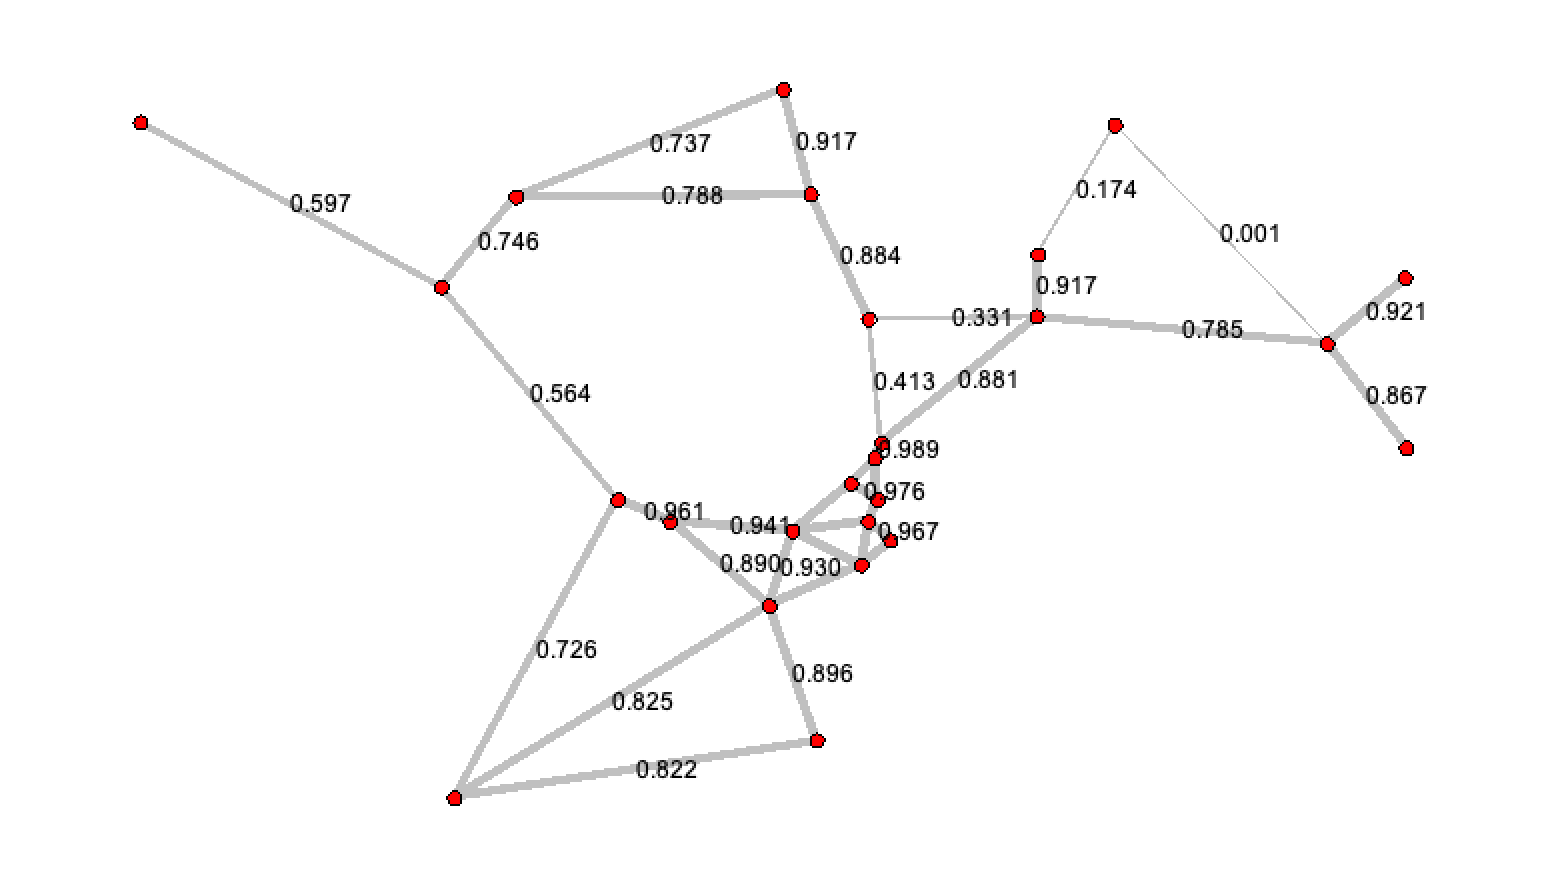
\includegraphics[width=0.45\textwidth]{img/gabriel}}
}
\caption{Comparison of graph construction methods using a sample of 25 nodes. Each method results in different connectivity patterns, affecting the subsequent clustering and route formation.}
\label{fig:graph_examples}
\end{figure}

\section{Clustering Graph Representation of IZTECH}
\label{sec:clustering_graph}

Once the various graph representations were constructed, we applied clustering algorithms to partition the nodes (students) into clusters, representing potential bus routes. The clustering phase is critical for identifying cohesive groups of students who can be efficiently transported together.

\subsection{Clustering Complete Graph Representation}
\label{subsec:clustering_complete}

Clustering the complete graph representation presents unique challenges due to its dense connectivity. Our implementation applies multiple clustering algorithms to the complete graph, each configured to respect the bus capacity constraints:

\begin{itemize}
    \item Minimum cluster size: 10 students (minimum efficient bus occupancy)
    \item Maximum cluster size: 50 students (maximum bus capacity)
\end{itemize}

We primarily utilized the Leiden algorithm (see Section~\ref{subsec:LeidenAlgorithm}), which optimizes modularity to find densely connected communities with its refinement phase ensuring well-connected clusters. The algorithm was configured with adaptive resolution to produce balanced clusters.

The clusters from the complete graph often required post-processing to merge small communities and split oversized ones, ensuring adherence to the capacity constraints. This post-processing uses geographic proximity to guide the merging and splitting operations, prioritizing the combination of communities that are spatially close while ensuring each resulting community remains within the capacity limits.

\subsection{Clustering Sparse Graph Representation}
\label{subsec:clustering_sparse}

The sparse graph representations required different clustering approaches due to their reduced connectivity. Our implementation adaptively configures the clustering algorithms based on the graph type.

For Delaunay and Gabriel graphs, we utilized the Spectral clustering algorithm (see Section~\ref{subsec:SpectralClustering}), which uses the eigenvalues and eigenvectors of the graph Laplacian to perform dimensionality reduction before clustering.

For the K-Nearest Neighbors graph, we found that the MVAGC (Multi-view Anchor Graph-based Clustering) algorithm performed especially well. As described in Section~\ref{subsec:MVAGC}, this algorithm constructs multiple views of the graph and integrates them through an anchor graph representation. Our configuration included approximately 500 anchor points, higher-order filtering for smooth community boundaries, and importance sampling to improve anchor diversity.

All clustering approaches were evaluated based on their ability to produce balanced clusters that minimize transportation costs while adhering to the vehicle capacity constraints.

% Placeholder for Clustering Example Visualization
\begin{figure}[!htbp]
\centering
\subfigure[Spectral Clustering]{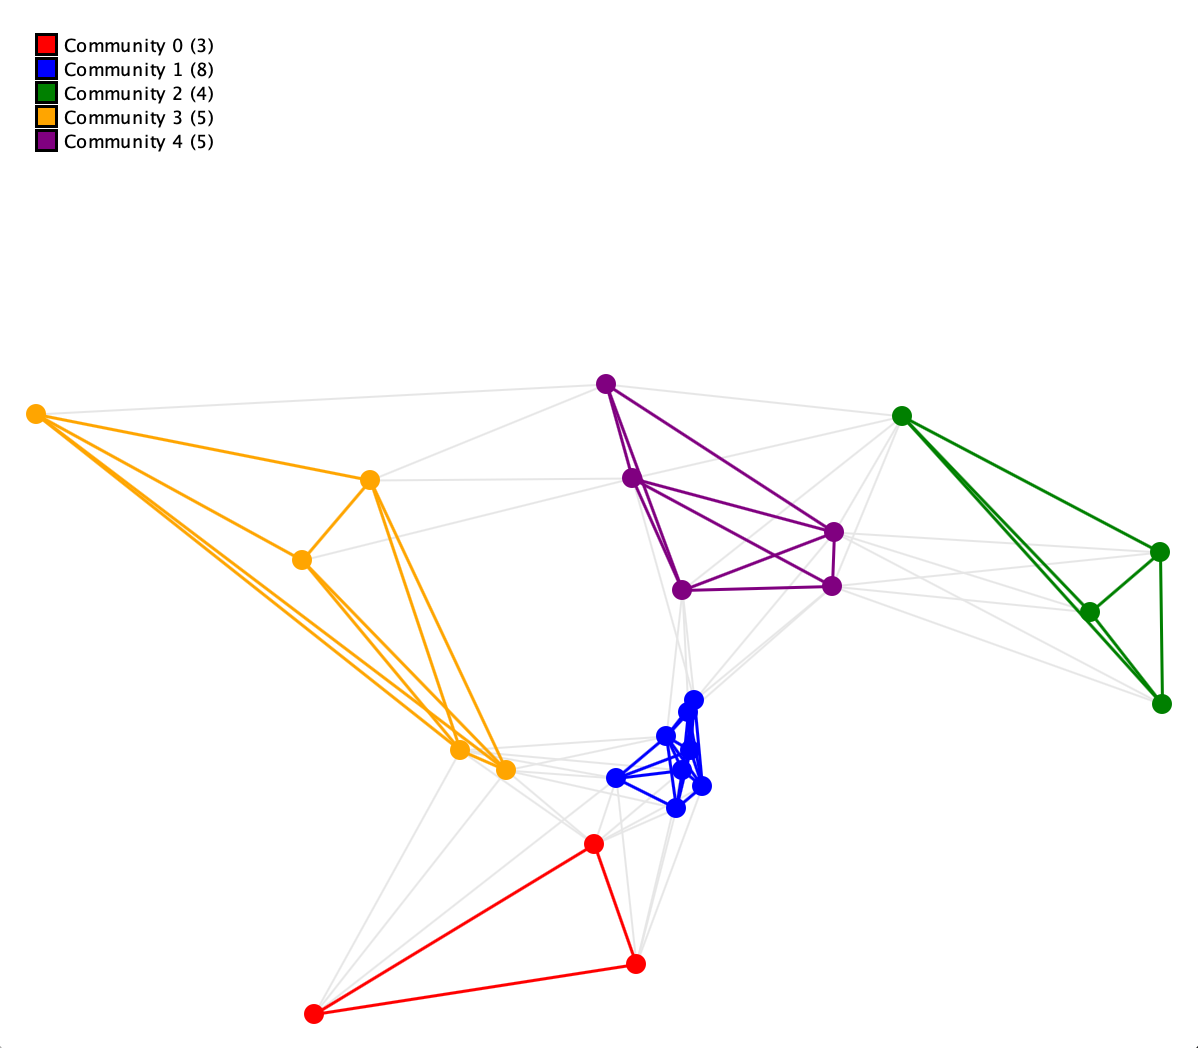
\includegraphics[width=0.32\textwidth]{img/spectral}}
\subfigure[Leiden Algorithm]{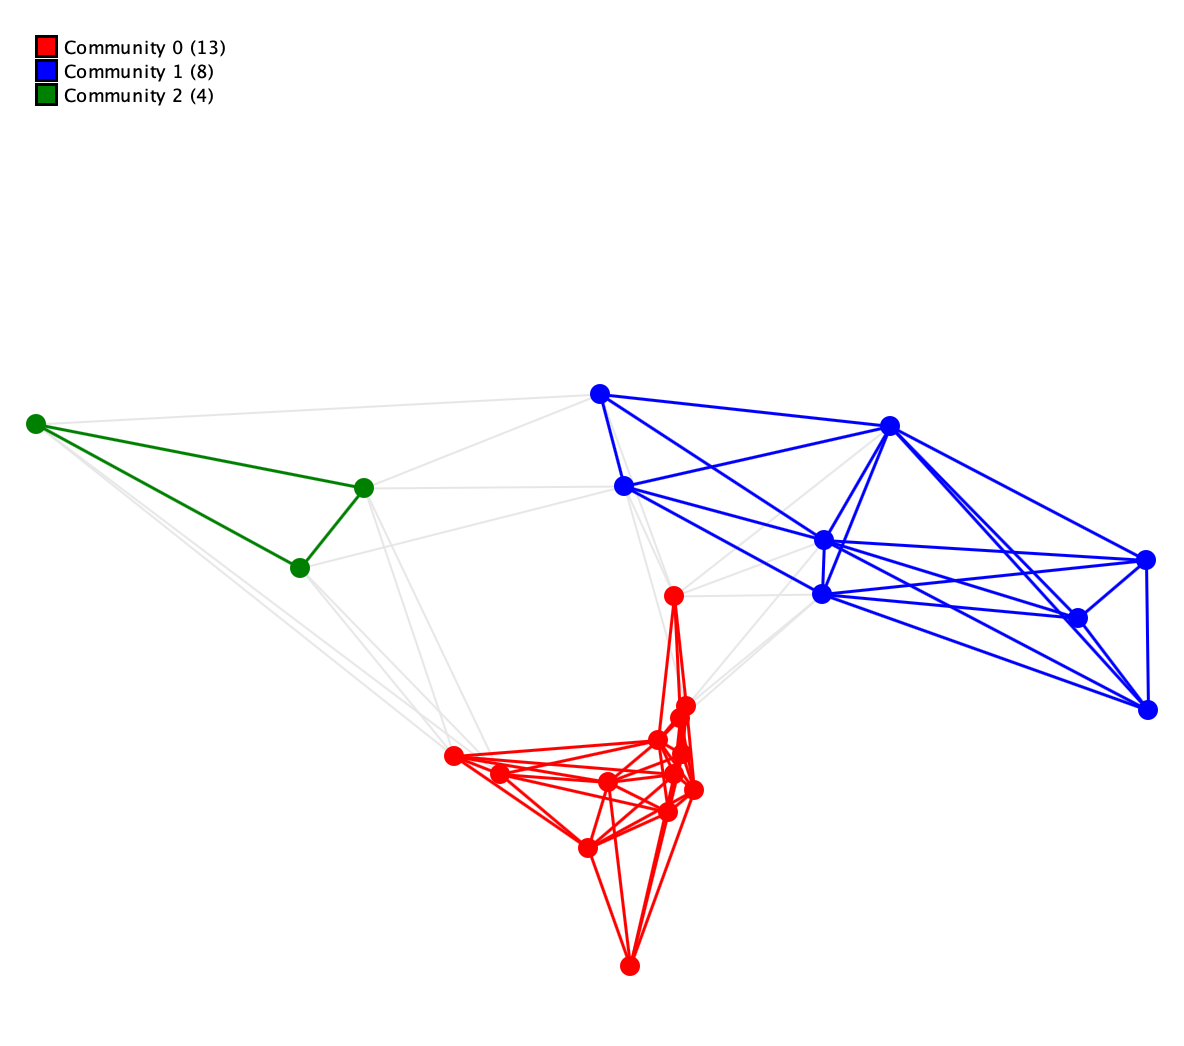
\includegraphics[width=0.32\textwidth]{img/leiden}}
\subfigure[MVAGC]{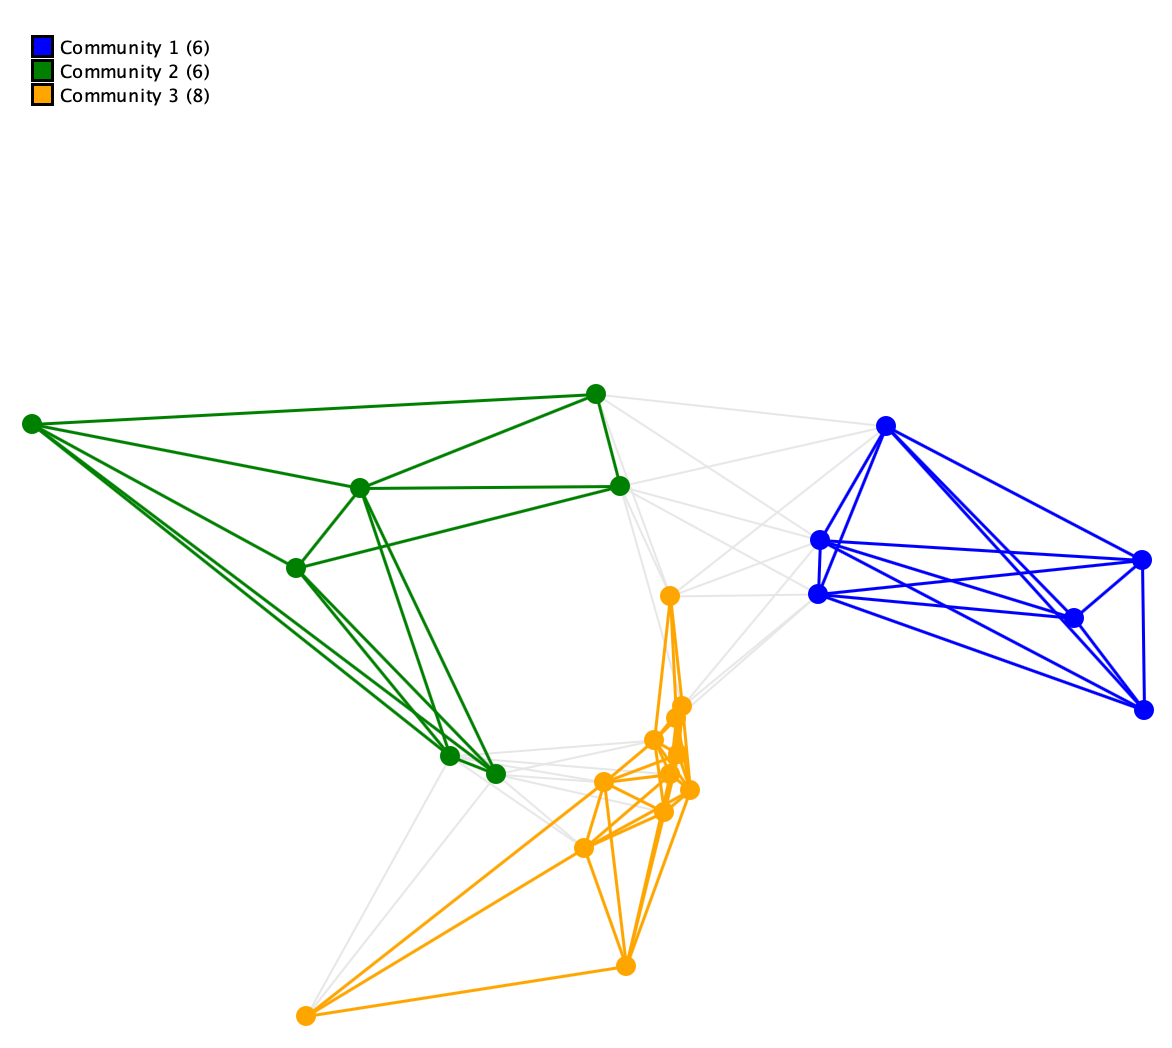
\includegraphics[width=0.32\textwidth]{img/mvagc}}
\caption{Results of applying different clustering algorithms to the graph representations. Each color represents a distinct cluster of student locations, corresponding to potential bus routes prior to capacity constraint adjustments.}
\label{fig:clustering_example}
\end{figure}

\section{Robustness for Clustering Graph Representation of IZTECH}
\label{sec:robustness}

% Empty section as requested, just the title placeholder

\section{Evaluation Framework and Route Mapping}
\label{sec:evaluation}

Applying each clustering algorithm to each graph type yields multiple potential partitionings. These were evaluated to find the most effective combinations based on practical transportation logistics, focusing on fuel efficiency and vehicle capacity utilization.

\subsection{Evaluation Metrics}
Key metrics used for evaluation included:
\begin{itemize}
    \item \textbf{Total Estimated Fuel Consumption:} Based on optimized routes within each cluster.
    \item \textbf{Number of Clusters/Routes:} Total buses required.
    \item \textbf{Capacity Constraint Adherence:} Checking if cluster sizes are within [10, 50].
    \item \textbf{Vehicle Type Allocation:} Assigning minibuses (max 25) or buses (max 50) efficiently.
\end{itemize}

\subsection{Mapping Clusters to Bus Routes}
Raw clusters were processed to ensure compliance with capacity constraints:
\begin{enumerate}
    \item \textbf{Cluster Size Check:} Verify $10 \leq |C| \leq 50$.
    \item \textbf{Handling Small Clusters ($|C| < 10$):} Merge with nearby clusters where feasible.
    \item \textbf{Handling Large Clusters ($|C| > 50$):} Split into multiple valid sub-routes.
    \item \textbf{Vehicle Assignment:} Assign minibus ($10 \leq |C| \leq 25$) or bus ($26 \leq |C| \leq 50$).
\end{enumerate}

This evaluation and mapping process allows for comparing the practical effectiveness of different graph and clustering strategies.

\section{Implementation Details}
\label{sec:implementation}

The described methodology was implemented using the Java programming language (JDK 17), with Apache Maven managing project dependencies. Several key libraries facilitated the graph construction, clustering, geospatial operations, and data handling:
\begin{itemize}
    \item \textbf{JGraphT:} Employed for core graph data structures, representing student locations as nodes and connections as edges \cite{jgrapht}.
    \item \textbf{GeoTools and JTS Topology Suite:} Utilized for handling geographical coordinates, performing spatial calculations, and constructing geometric graphs \cite{geotools, jts}.
    \item \textbf{Apache Commons CSV:} Used for reading student location data and writing results \cite{commonscsv}.
    \item \textbf{Efficient Java Matrix Library (EJML):} Provided necessary matrix operations, particularly eigenvalue decomposition required for Spectral Clustering \cite{ejml}.
\end{itemize}

The analysis relied on coordinate data for student locations. Edge weights representing estimated fuel costs were calculated using distance information derived from the geospatial libraries and standard vehicle fuel efficiency models. Data might have been sourced or cross-referenced with external datasets from OpenStreetMap.

% Commenting out the example algorithm from the template
% \begin{algorithm}
% \begin{algorithmic}[1]
% \STATE generate random number $n \in [l, u]$
% \WHILE{$n \neq 42$}
% \IF{today is Tuesday}
% \STATE print(42)
% \ENDIF
% \ENDWHILE
% \RETURN best solution found so far
% \end{algorithmic}
% \caption{Basic Algorithm($l, u$)}
% \label{alg:example_alg}
% \end{algorithm}



